% !TEX root = ../IS.tex
\chapter{Description of Software}
\section{AI Model}
\subsection{Simulation Model}
For this thesis, a 2D, turn-based role-playing game (RPG) was created. In an RPG, players are given a list of possible actions they may take on their turn. These actions consist of, but are not limited to: attacking (usually with a melee weapon), using magical spells (of both offensive and defensive varieties), and using items (to either heal players or otherwise make them more powerful). These choices are tied to the character the player controls, along with their character stats. A thief character may be faster and more nimble, but may also be weaker and unable to use magical spells. A knight character could be stronger and better defended with their armor, but also slower and easier for opponents to hit. With regards to player actions and choices, the thief may be able to steal items, while the knight may be able to block attacks with a shield. This is the ``role-playing'' aspect of the game: the player chooses their actions based on the role of their in-game character.\\

\begin{figure}[H]
  \centering
  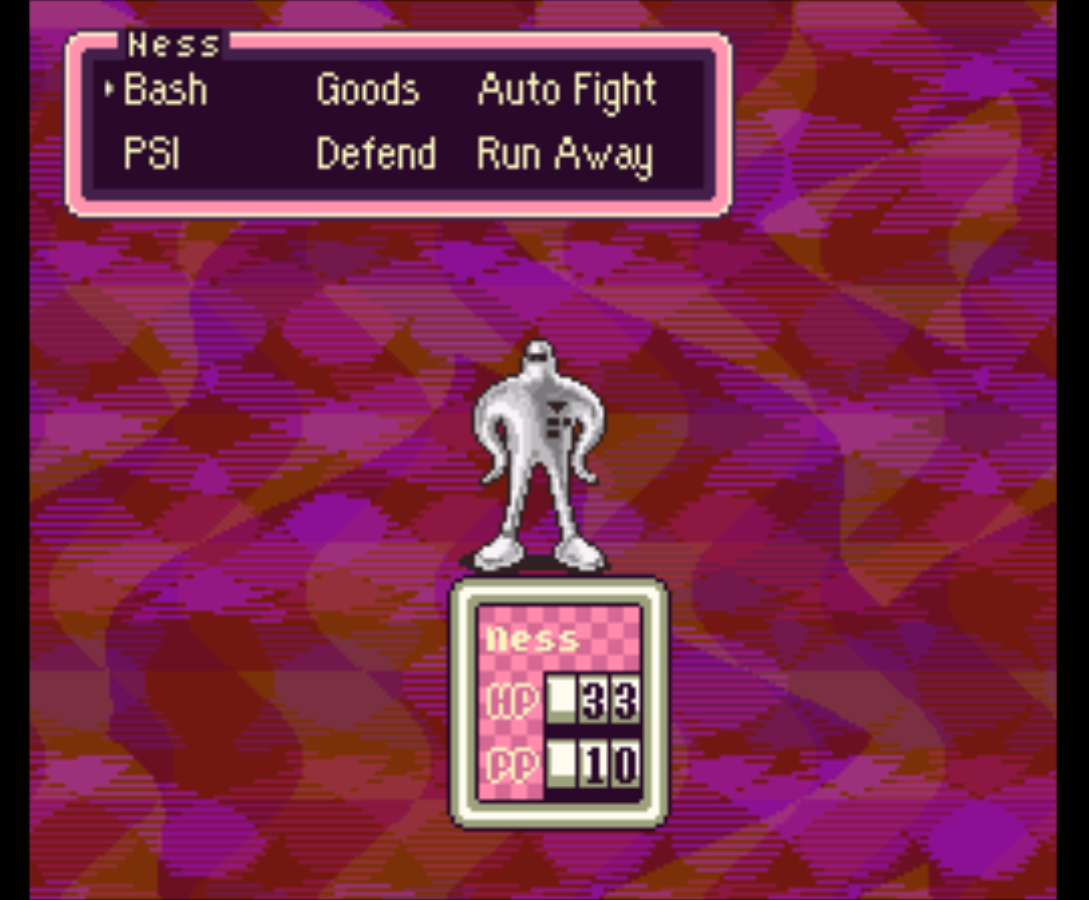
\includegraphics[width=9cm]{figures/Earthbound.png}
  \caption{A screenshot of a battle from the turn-based role-playing game \textit{Earthbound}.}
  \label{fig:Earthbound}
\end{figure}

For instance, observe the battle shown in Figure \ref{fig:Earthbound} from the game \textit{Earthbound}. The computer opponent is shown in the center of the screen. At the top, the actions available to the player are listed. Players have the choice of making a melee attack (Bash), casting a magical spell (PSI), using an item (Goodies), or reducing damage taken (Defend). Players can also select Auto Fight to have the computer make all the choices for them, or they can Run Away and escape from the battle. At the bottom, the hit points (HP) and psychic points (PP) of the character are shown - these correspond to the character's health and their magical abilities.

Specific to turn-based RPGs, the player has as much time as they want to decide on their strategy. This is in contrast to an action RPG, where combat takes place in real-time. Generally, action RPGs use 3D environments to better accommodate the real-time battles, but this is not always the case. In the game created for this thesis, a turn-based approach is better suited because it emphasizes player strategy. Action RPGs may have similar lists of commands and actions, but these actions frequently have a corresponding skill component. Take for example a basic attack. In a turn-based RPG, this action requires little from the player: they select that choice from a list, and their in-game character attacks the opposing player. Depending on the game, this attack may or may not be successful - the opponent could dodge or block the hit - but the success or failure is determined by the game through the stats both players - if for instance a character is nimble enough to dodge, or defensive enough to block a strike. An action RPG, on the other hand, determines whether an attack misses or hits through hit-boxes. A hit-box is a hidden area tied to some in-game object; when hit-boxes intersect, something happens depending on the types of objects. For this example, an attack would be successful if the hit-box of the character's attack (their sword, fist, magic spell, etc.) intersects with the hit-box of their opponent's body. The attack would fail if these hit-boxes do not intersect. Thus, the overall success of a character in an action RPG is dependent on a player's skill in making hitboxes collide. This type of gameplay does not lend itself well to game theory analysis, as a player could make all the right decisions but still lose from lack of skill.\\

Similarly, the game presented in this thesis is a two-dimensional game. With a turn-based RPG, since the gameplay involves choosing actions from a list, the only difference between a 2D and a 3D turn-based RPG is the graphical quality. A 2D game uses sprites, while 3D games use polygonal models. A two-dimensional game was chosen to simplify development.\\

To begin building an AI model, we first create a simulation of the game. The simulation has two players, each with 25 health points (HP). Both players have two possible actions per turn, which are randomly selected: attack the other player, reducing their opponents HP by 5 points, or heal themselves, increasing their HP by 4 points. Players can not heal above their starting value of 25 HP; any extra health points are discarded. Each action has a 50\% chance of occurring. The game runs until one player's HP is reduced to 0. The total number of turns and the sequence of actions are recorded into a CSV file. After running 4500 simulations, the data is imported into Matlab. A subset of the games are used as a training set for a decision tree, which predicts the player that wins the game.\\

\begin{figure}[H]
  \centering
  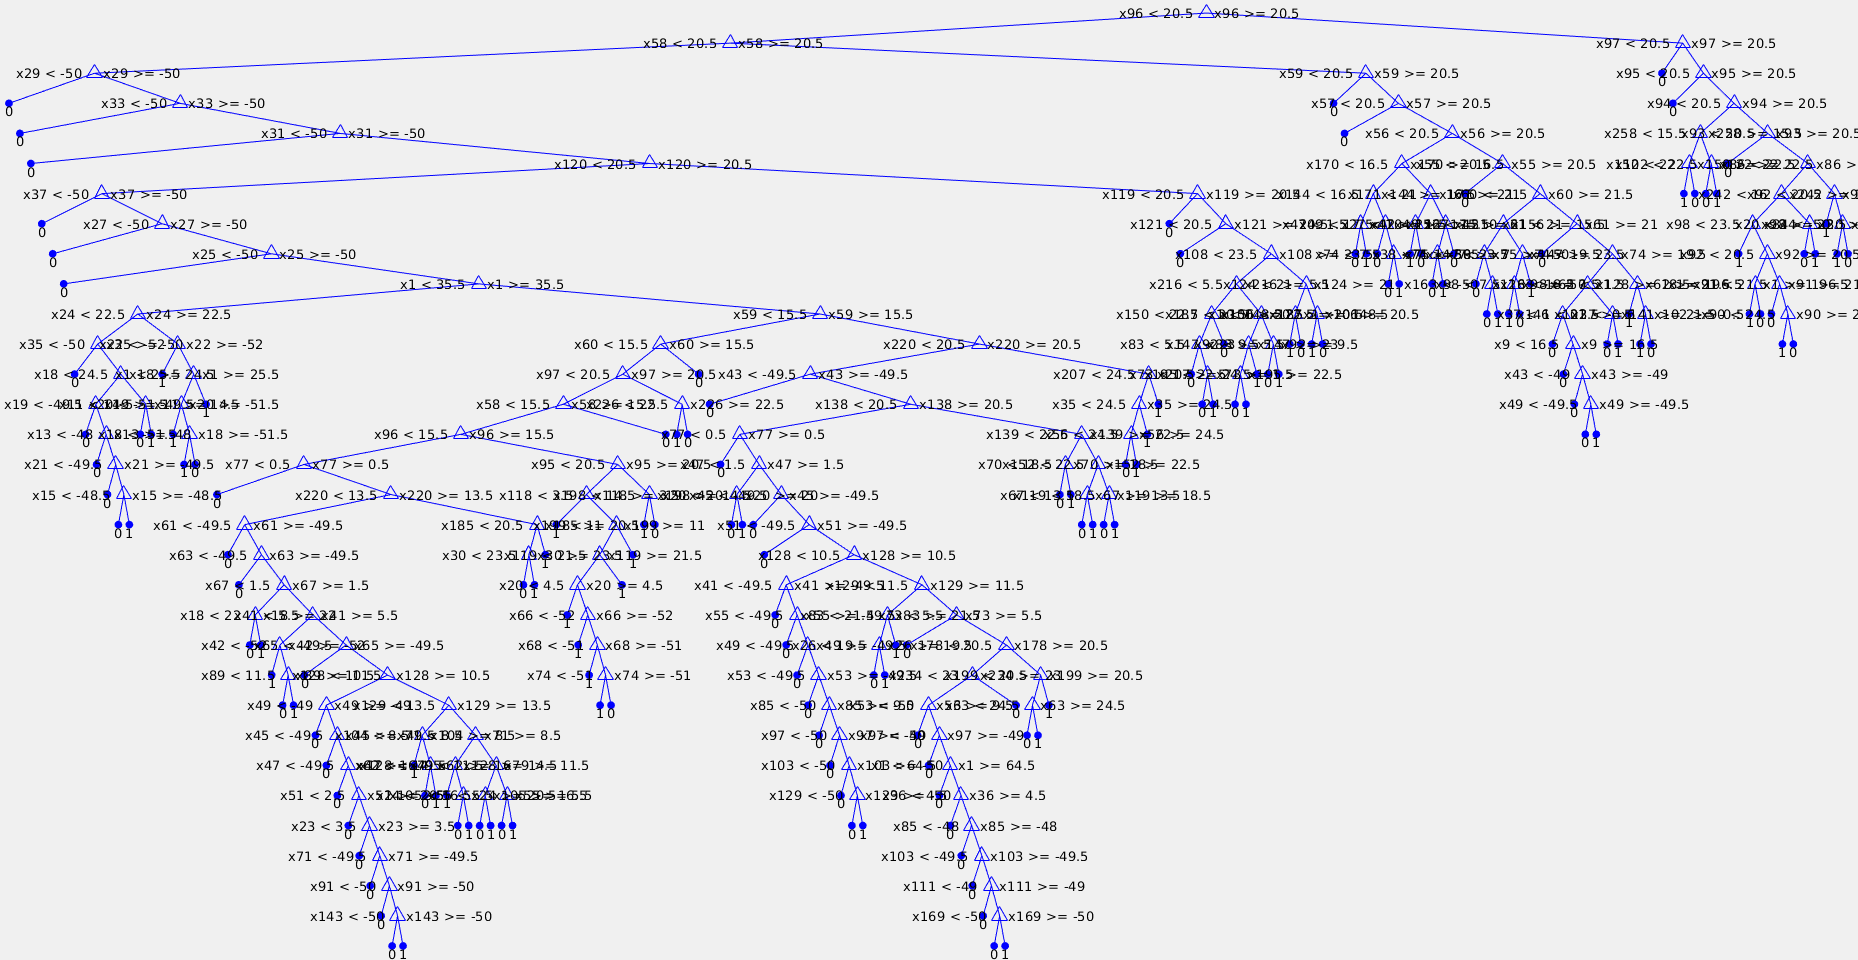
\includegraphics[width=13cm]{figures/firstDecisionTree.png}
  \caption{The decision tree generated from 4000 simulations of the game. This tree predicts 0 when player 1 wins and 1 when player 2 wins.}
  \label{fig:decisionTree1}
\end{figure}

However, this method is inconclusive, for a number of reasons. Firstly, the decision tree includes a large number of branches, as seen in Figure \ref{fig:decisionTree1}. Secondly, the actual criteria evaluated at each branch of the tree is different for each game. Aside from the first column, which contains the total number of turns in the game, and the second column, which contains the starting HP of player 1, the values in any particular column differ from game to game. For instance, the root node uses the value in column 96 as its classifier. In one game, column 96 may contain a HP value for player 2. In another, longer game, that column may contain a HP value for player 1. Thirdly, the individual games contain numerous streaks: a longer game is not the result of better strategy, but is instead caused by streaks where both players choose to heal on their turns. Players in these streaks reach HP levels near the 25 HP cap, effectively resetting the game.

The lack of consistency along columns is most likely the largest detriment to this model. Decision trees work best when classifying problems on specific attributes; if the attribute is different at column 96 from one game to another, the information gain at that column is meaningless. This is likely behind the sprawling nature of the decision tree itself. Without clear attributes to test, each split only has minuscule amounts of information gain.

\subsection{Extensive Tree Model}
A game theoretic angle is used on the second attempt. The HP of both players is reduced to 10, and two restrictions are added on healing: a player can not heal when they have full health, and a player can only heal themselves twice. With these new rules in place, we create an extensive-form tree for the new game.\\

\begin{figure}[H]
  \centering
  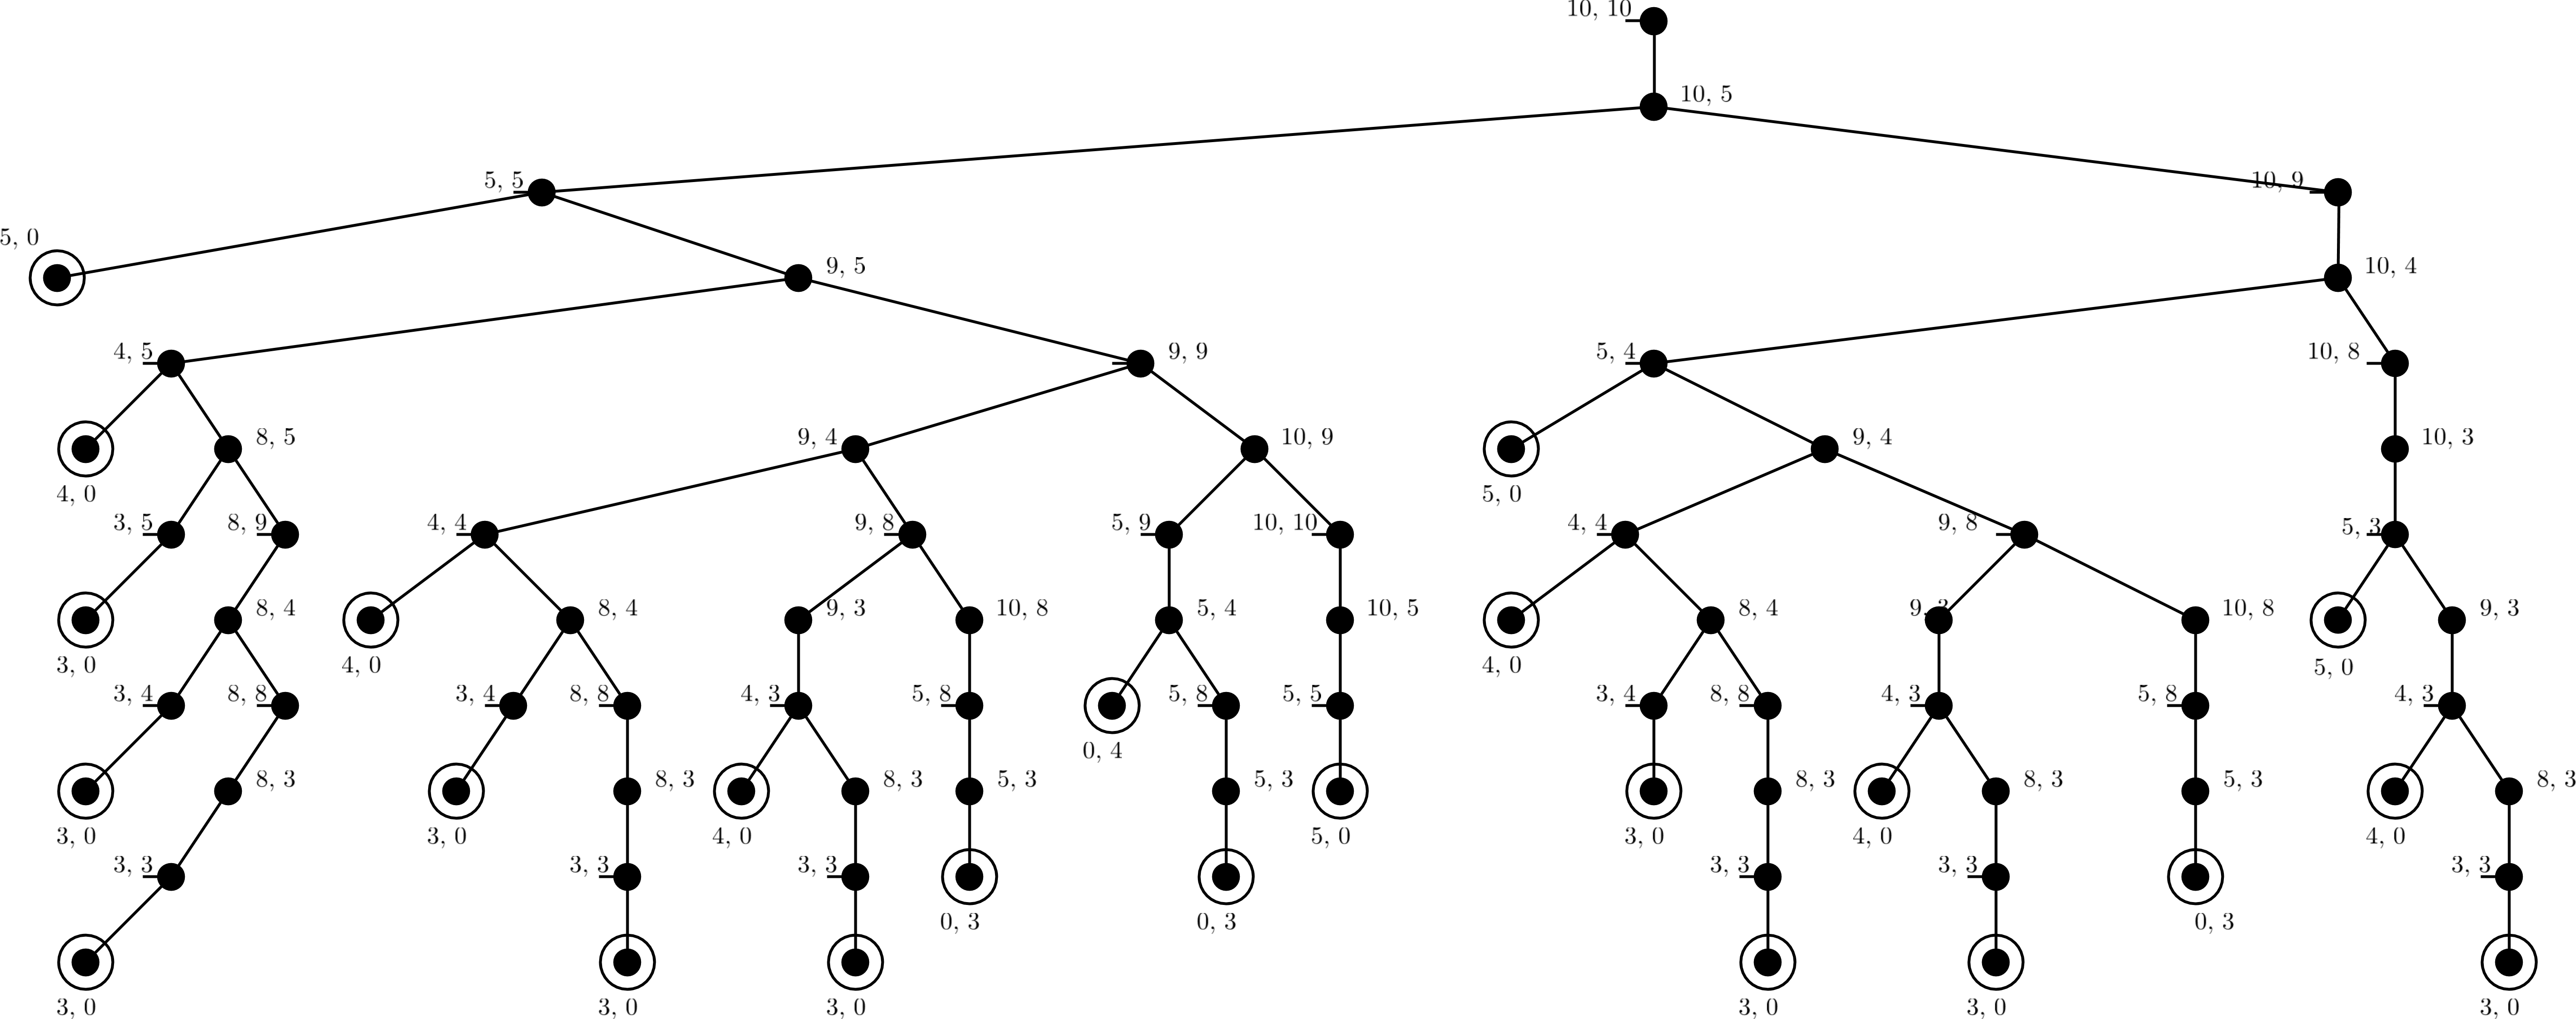
\includegraphics[width=15cm]{figures/GameTree.png}
  \caption{The extensive-form tree for a simplified game. Each player has 10 HP, and can only heal themselves twice.}
  \label{fig:gameTree}
\end{figure}

In Figure \ref{fig:gameTree}, player 1's nodes are denoted by a small dash to the left of the node. The HP values of both players are recorded at each node. Leaf nodes where player 1 wins are enclosed in a circle, and leaf nodes where player 2 wins are enclosed in a diamond. There are 24 outcomes for this game; of these, only 4 of them result in a win for player 2, while the other 20 result in wins for player 1. In fact, with optimal play, player 1 always wins in this game.\\

\begin{figure}[H]
  \centering
  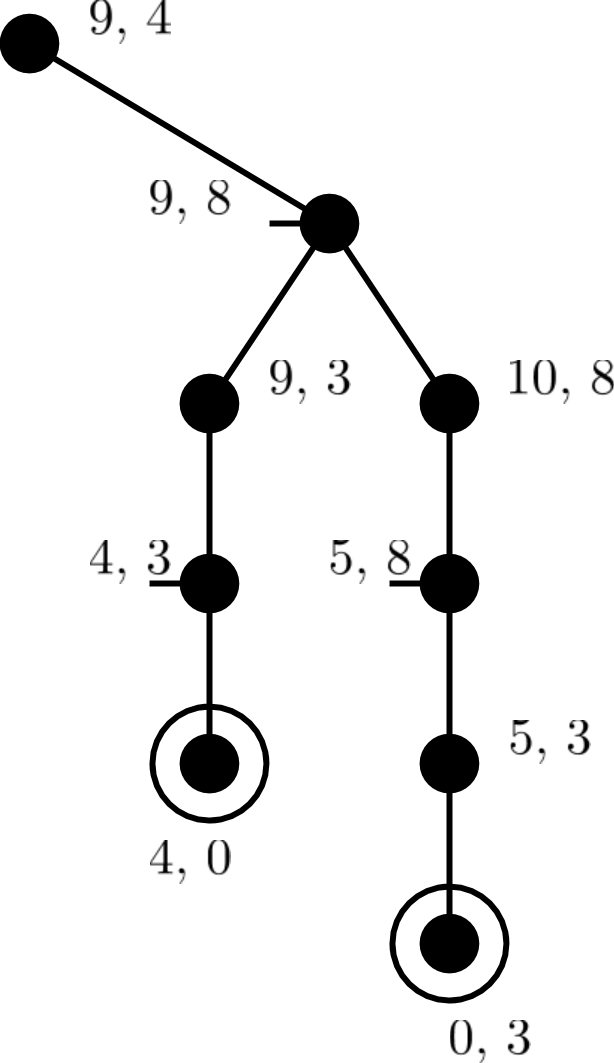
\includegraphics[width=4cm]{figures/GameSubtree.png}
  \caption{A subtree of the extensive-form representation}
  \label{fig:gameSubtree}
\end{figure}

For example, in this subtree, both player 1 and 2 have a winning outcome. However, the critical decision is made by player 1. Thus, in any game which reaches this subtree, player 1 chooses to attack on their turn, since that choice leads to their victory.\\

\begin{figure}[H]
  \centering
  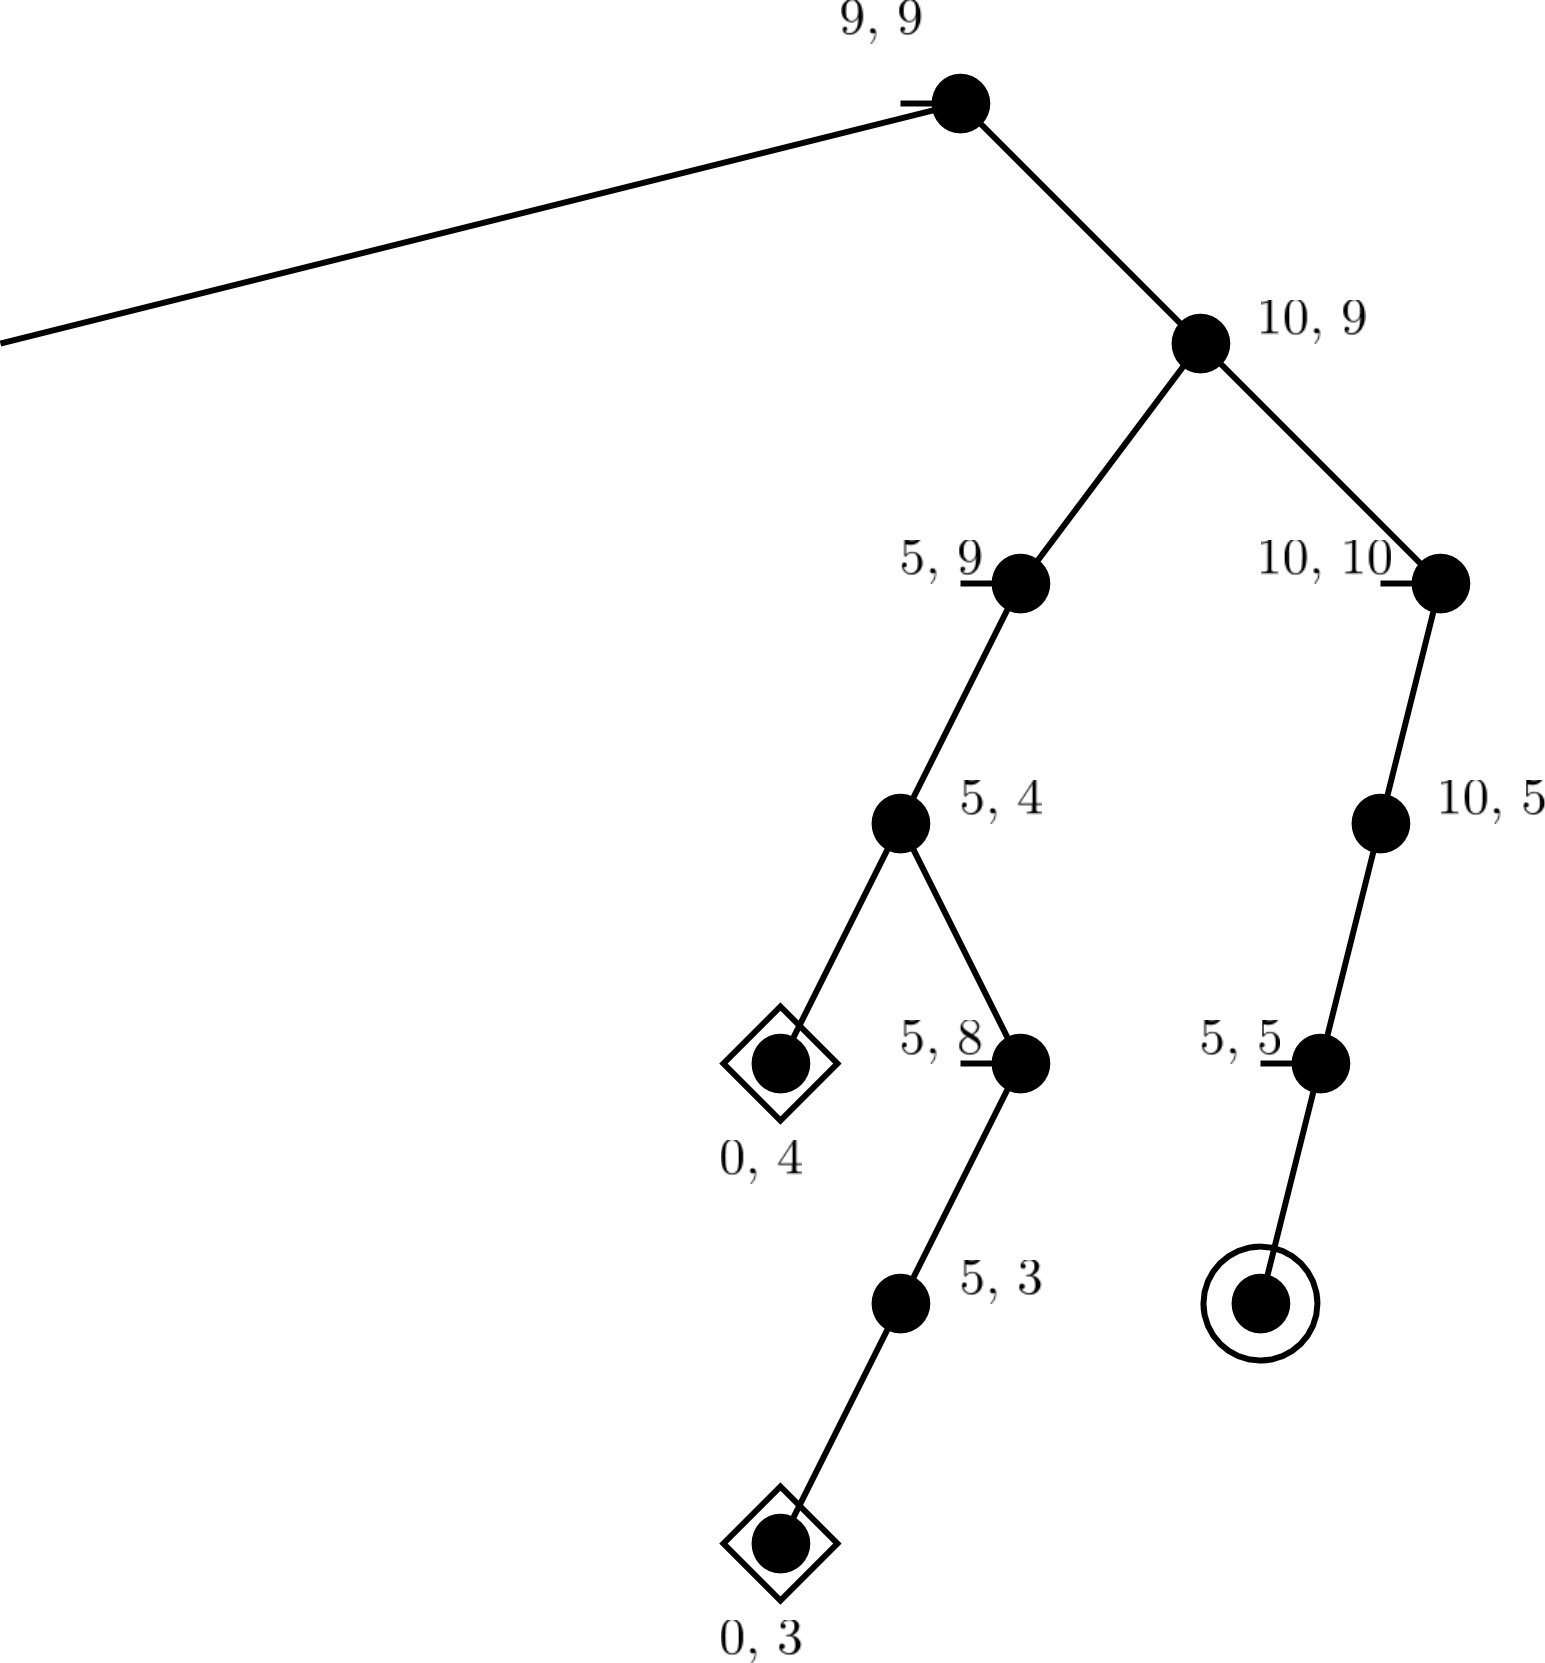
\includegraphics[width=9cm]{figures/GameSubtree2.png}
  \caption{A larger subtree of the extensive-form representation}
  \label{fig:gameSubtree2}
\end{figure}

The remainder of player 2's winning outcomes can be seen in the subtree in Figure \ref{fig:gameSubtree2}. At the root node of this subtree, player 1 is making their choice. If they choose to heal, the game moves into the right child. Player 2's first choice on the right child's subtree either results in a win (if player 2 attacks) or a loss (if player 2 heals). Thus, an intelligent player 2 would always attack at this stage, since it is a guaranteed win. However, if player 1 knows that this is a guaranteed win for their opponent, player 1 can avoid this threat by attacking instead of healing at the root node.\\

In this limited model, it is clear that healing is not a viable strategy. The HP recovered by one player is not enough to offset the damage dealt by their opponent. At the most, choosing to heal only delays the inevitable.\\

In the four paths where player 2 won, there is a node where player 1 chose to heal from 9 HP to 10 HP. Since the normal amount of HP recovered by healing is 4 HP, we can see that player 1 is wasting potential HP by using one of their turns to heal when their HP is already close to the HP cap. We may infer that, in games with larger HP caps, the same effects would appear. It is much more useful for a player to heal when their HP is closer to zero.\\

Now that some patterns in the game are identified, we expand the game and build a prototype using Python and the pygame library.

\section{Game Engine}
Python was chosen as the development language for this game. Python is an extremely portable language: anyone with Python installed can run the code. Python also has a robust library for two-dimensional games called pygame, which was essential in creating this game. Specifically, Python 3 was used for better compatibility with the pygame library and for the copy() function for arrays.

\subsection{The pygame Library}
The pygame library provides a number of Python functions that are useful in creating a two-dimensional video game. The library was originally created in 2001 to combine Python with SDL (Simple DirectMedia Layer), a library of multimedia controls written for C \cite{shinners}. pygame can utilize a variety of different graphics libraries, including OpenGL, DirectX, the Linux frame buffer, and an ASCII art backend \cite{shinners}. The pygame library is supported by numerous operating systems, and the core functions of pygame use highly optimized C or assembly code.\\

At the top level, pygame controls the initialization and exiting of its various modules, particularly the pygame.display module which renders the game. pygame features two functions to update a display window, pygame.display.flip() and pygame.display.update(). display.flip() works with two separate arrays, containing the pixel data for the window in which the game operates. One array is displayed on the screen, while the other array is used to record changes made to the on-screen image. Once all changes are made, display.flip() swaps these arrays, or ``buffers,'' by copying all the data from one array into the other. The buffer that recorded changes is now displayed on-screen, while the buffer that was displayed can now be used to record further changes. display.update() is an optimized version of flip() that takes as an argument a rectangle or a sequence of rectangles. These rectangles correspond to the areas of the display that need to be updated. For instance, passing the coordinates of a rectangle over a game's scoreboard only updates the scoreboard. With this function, large sections of the pixel array do not need to be copied from one buffer to another, speeding up the rendering process.\\

The two main objects in pygame are the Surface object and the sprite object. Surfaces can be changed with pygame to alter various attributes. For instance, the alpha value, or the transparency of the surface, can be changed with set\_alpha(). The individual color values can be converted to integers and vice versa with the map\_rgb() and unmap\_rgb() functions, respectively. This allows for pygame to store colors as a single number, rather than a tuple of integers. Surfaces are mostly used to load image files and to create backgrounds for the game. Sprites, on the other hand, are used for the actual in-game objects, such as enemies, player characters, and projectiles. Sprites can be stored in a Group object, that can be used to separate sprites by different purposes. Each sprite draws its image to a Surface, provided that it has a Surface.image and Surface.rect attribute.\\

Once a sprite or surface is created with an image, pygame can also perform graphical transformations on that image. The pygame.transform module has functions to flip, rotate, and scale an image. Another pygame feature is the ability to do collision detection on sprites and rectangles.\\

For the actual gameplay of a pygame program, there are also modules for joystick, mouse, and keyboard controls. A sound mixer module allows audio tracks to be played in the game, and the pygame.time module controls the framerate of the game.

\subsection{Gameplay Design}
For the expanded version of the game, several things were changed from the game in Figure \ref{fig:gameTree}. Two additional choices were added: Parry and Strong Attack. With Parry, the player enters a guarded stance until their next turn; this player will be referred to as the defending player. If, before their next turn, their opponent attacks them, the defending player counter-attacks. The defending player loses no HP, and the player who attacked them loses 3 HP from the counter-attack. A Strong Attack does more damage than a regular attack (7 HP vs 5 HP), but has a chance to miss the opponent completely and do no damage. Additionally, a Strong Attack is unaffected by Parry; if a player is Parrying and their opponent uses a strong attack, the parry is unsuccessful and the defending player suffers 7 HP of damage.

The two players in the game begin with 25 HP each, and are able to heal twice per game. These values are stored in a PlayerAvatar class. This class also stores the type of AI used for the computer player. The class has a helper function, which is called from within the main game loop. This helper function checks which AI model is used, then calls that model's respective function.

Seven different AI models were created. In all models, the AI checks to see if any healing turns remain; if not, the AI defaults to a normal attack. Three of the models rely on a random number generator. The first, the limitedRandomAI() function, chooses randomly to attack or heal, with a 50/50 chance of either, but will attack instead if the AI has already healed itself twice. The second model, randomAI(), has a 25\% chance of attacking, healing, parrying, or using a strong attack. Again, if the random number generator indicates the AI should heal, but all healing turns have been used, the AI does a normal attack instead.